
\section{Exploring institutionally curated cancer genomics data}\label{exploring-institutionally-curated-cancer-genomics-data}}


\subsection{The Cancer Genome Atlas}\label{the-cancer-genome-atlas}}

An overview of Bioconductor's resource for the Cancer
Genome Atlas (TCGA) is easy to obtain, with the
curatedTCGAData package.

\begin{shaded}
\begin{verbatim}
library(curatedTCGAData)
tcgatab = curatedTCGAData(version="2.1.1")
\end{verbatim}
\end{shaded}
%\begin{Shaded}
%\begin{Highlighting}[]
%\KeywordTok{library}\NormalTok{(curatedTCGAData)}
%\NormalTok{tcgatab =}\StringTok{ }\KeywordTok{curatedTCGAData}\NormalTok{(}\DataTypeTok{version=}\StringTok{"2.1.1"}\NormalTok{)}
%\end{Highlighting}
%\end{Shaded}

Records obtained for adrenocortical carcinoma (code ACC) are in Table \ref{tab:tab-lktab}.

\begin{table}

\caption{\label{tab:tab-lktab}Records returned by curatedTCGAData::curatedTCGAData(), filtered to those pertaining to adrenocortical carcinoma.}
\centering
\begin{tabular}[t]{lllll}
\toprule
  & ah\_id & title & file\_size & rdataclass\\
\midrule
1 & EH4737 & ACC\_CNASNP-20160128 & 0.8 Mb & RaggedExperiment\\
2 & EH4738 & ACC\_CNVSNP-20160128 & 0.2 Mb & RaggedExperiment\\
3 & EH4740 & ACC\_GISTIC\_AllByGene-20160128 & 0.2 Mb & SummarizedExperiment\\
4 & EH4741 & ACC\_GISTIC\_Peaks-20160128 & 0 Mb & RangedSummarizedExperiment\\
5 & EH4742 & ACC\_GISTIC\_ThresholdedByGene-20160128 & 0.2 Mb & SummarizedExperiment\\
\addlinespace
6 & EH4744 & ACC\_Methylation-20160128\_assays & 239.2 Mb & SummarizedExperiment\\
7 & EH4745 & ACC\_Methylation-20160128\_se & 6 Mb & RaggedExperiment\\
8 & EH4747 & ACC\_Mutation-20160128 & 0.7 Mb & SummarizedExperiment\\
9 & EH4748 & ACC\_RNASeq2Gene-20160128 & 2.7 Mb & SummarizedExperiment\\
10 & EH4750 & ACC\_RPPAArray-20160128 & 0.1 Mb & SummarizedExperiment\\
\addlinespace
414 & EH8118 & ACC\_miRNASeqGene-20160128 & 0.2 Mb & SummarizedExperiment\\
415 & EH8119 & ACC\_RNASeq2GeneNorm-20160128 & 5.4 Mb & SummarizedExperiment\\
\bottomrule
\end{tabular}
\end{table}

Various conventions are in play in this table. The ``title'' field is
of primary concern. The title string can be decomposed into
substrings with interpretation
\texttt{{[}tumorcode{]}\_{[}assay{]}-{[}date{]}\_{[}optional codes{]}}. The column \texttt{ah\_id} will be
explained in section \ref{hubs}, and entries in column
\texttt{rdataclass} will be discussed in section \ref{class} below.


\subsubsection{Tumor code resolution}\label{tumor-code-resolution}}

There are 33 different tumor types available in TCGA. The
decoding of tumor codes for the first ten in alphabetical order is
provided in Table \ref{tab:tab-deco}.

\begin{table}

\caption{\label{tab:tab-deco}Decoding TCGA tumor code abbreviations.}
\centering
\begin{tabular}[t]{ll}
\toprule
Code & Tumor.Type\\
\midrule
ACC & Adrenocortical Carcinoma\\
BLCA & Bladder Urothelial Carcinoma\\
BRCA & Breast Invasive Carcinoma\\
CESC & Cervical Squamous Cell Carcinoma and Endocervical Adenocarcinoma\\
CHOL & Cholangiocarcinoma\\
\addlinespace
CNTL & Controls\\
COAD & Colon Adenocarcinoma\\
DLBC & Lymphoid Neoplasm Diffuse Large B-cell Lymphoma\\
ESCA & Esophageal Carcinoma\\
FPPP & FFPE Pilot Phase II\\
\addlinespace
GBM & Glioblastoma Multiforme\\
HNSC & Head and Neck Squamous Cell Carcinoma\\
KICH & Kidney Chromophobe\\
KIRC & Kidney Renal Clear Cell Carcinoma\\
KIRP & Kidney Renal Papillary Cell Carcinoma\\
\addlinespace
LAML & Acute Myeloid Leukemia\\
LCML & Chronic Myelogenous Leukemia\\
LGG & Brain Lower Grade Glioma\\
LIHC & Liver Hepatocellular Carcinoma\\
LUAD & Lung Adenocarcinoma\\
\addlinespace
LUSC & Lung Squamous Cell Carcinoma\\
MESO & Mesothelioma\\
MISC & Miscellaneous\\
OV & Ovarian Serous Cystadenocarcinoma\\
PAAD & Pancreatic Adenocarcinoma\\
\addlinespace
PCPG & Pheochromocytoma and Paraganglioma\\
PRAD & Prostate Adenocarcinoma\\
READ & Rectum Adenocarcinoma\\
SARC & Sarcoma\\
SKCM & Skin Cutaneous Melanoma\\
\addlinespace
STAD & Stomach Adenocarcinoma\\
TGCT & Testicular Germ Cell Tumors\\
THCA & Thyroid Carcinoma\\
THYM & Thymoma\\
UCEC & Uterine Corpus Endometrial Carcinoma\\
\addlinespace
UCS & Uterine Carcinosarcoma\\
UVM & Uveal Melanoma\\
\bottomrule
\end{tabular}
\end{table}


\subsubsection{Assay codes and counts}\label{assay-codes-and-counts}}

Assays performed on tumors vary across tumor types. For assay
types shared between
breast cancer, glioblastoma, and lung adenocarcinoma (code LUAD),
the numbers of tumor and normal samples available in curatedTCGAData
are provided in Table \ref{tab:tab-doassc}.

\begin{table}

\caption{\label{tab:tab-doassc}Numbers of assays available in TCGA on tumor and normal samples,
for breast cancer, glioblastoma, and lung adenocarcinoma.}
\centering
\begin{tabular}[t]{lrrrrrr}
\toprule
  & BRCA & BRCAnormal & GBM & GBMnormal & LUAD & LUADnormal\\
\midrule
CNASNP & 1089 & 1120 & 577 & 527 & 516 & 579\\
CNVSNP & 1080 & 1119 & 577 & 527 & 516 & 579\\
GISTIC\_AllByGene & 1080 & 0 & 577 & 0 & 516 & 0\\
GISTIC\_Peaks & 1080 & 0 & 577 & 0 & 516 & 0\\
GISTIC\_ThresholdedByGene & 1080 & 0 & 577 & 0 & 516 & 0\\
\addlinespace
Mutation & 988 & 5 & 283 & 7 & 230 & 0\\
RNASeq2Gene & 1093 & 119 & 153 & 13 & 515 & 61\\
RPPAArray & 887 & 50 & 233 & 11 & 365 & 0\\
RNASeq2GeneNorm & 1093 & 119 & 153 & 13 & 515 & 61\\
Methylation\_methyl27 & 314 & 29 & 285 & 0 & 65 & 24\\
\addlinespace
Methylation\_methyl450 & 783 & 102 & 140 & 14 & 458 & 34\\
\bottomrule
\end{tabular}
\end{table}


\subsubsection{An example dataset for RNA-seq from glioblastoma multiforme}\label{an-example-dataset-for-rna-seq-from-glioblastoma-multiforme}}

We obtain normalized RNA-seq data on primary tumor samples for GBM with

%\begin{Shaded}
%\begin{Highlighting}[]
%\NormalTok{gbrna =}\StringTok{ }\KeywordTok{TCGAprimaryTumors}\NormalTok{(}\KeywordTok{curatedTCGAData}\NormalTok{(}\StringTok{"GBM"}\NormalTok{, }
%    \StringTok{"RNASeq2GeneNorm"}\NormalTok{, }\DataTypeTok{dry.run=}\OtherTok{FALSE}\NormalTok{, }\DataTypeTok{version=}\StringTok{"2.1.1"}\NormalTok{))}
%\NormalTok{gbrna}
%\CommentTok{\#\# A MultiAssayExperiment object of 1 listed}
%\CommentTok{\#\#  experiment with a user{-}defined name and respective class.}
%\CommentTok{\#\#  Containing an ExperimentList class object of length 1:}
%\CommentTok{\#\#  [1] GBM\_RNASeq2GeneNorm{-}20160128: SummarizedExperiment with 18199 rows and 153 columns}
%\CommentTok{\#\# Functionality:}
%\CommentTok{\#\#  experiments() {-} obtain the ExperimentList instance}
%\CommentTok{\#\#  colData() {-} the primary/phenotype DataFrame}
%\CommentTok{\#\#  sampleMap() {-} the sample coordination DataFrame}
%\CommentTok{\#\#  \textasciigrave{}$\textasciigrave{}, \textasciigrave{}[\textasciigrave{}, \textasciigrave{}[[\textasciigrave{} {-} extract colData columns, subset, or experiment}
%\CommentTok{\#\#  *Format() {-} convert into a long or wide DataFrame}
%\CommentTok{\#\#  assays() {-} convert ExperimentList to a SimpleList of matrices}
%\CommentTok{\#\#  exportClass() {-} save data to flat files}
%\end{Highlighting}
%\end{Shaded}

\begin{shaded}
\begin{verbatim}
gbrna = TCGAprimaryTumors(curatedTCGAData("GBM",
     "RNASeq2GeneNorm", dry.run=FALSE, version="2.1.1"))
gbrna
## A MultiAssayExperiment object of 1 listed
##experiment with a user-defined name and respective class.
##Containing an ExperimentList class object of length 1:
[1] GBM_RNASeq2GeneNorm-20160128: SummarizedExperiment with 
##        18199 rows and 153 columns
##
## Functionality:
##experiments() - obtain the ExperimentList instance
##colData() - the primary/phenotype DataFrame
##sampleMap() - the sample coordination DataFrame
##`$`, `[`, `[[` - extract colData columns, subset, or experiment
####*Format() - convert into a long or wide DataFrame
assays() - convert ExperimentList to a SimpleList of matrices
##exportClass() - save data to flat files
\end{verbatim}
\end{shaded}

R functions defined in Bioconductor packages can operate on the variable \texttt{gbrna} to
retrieve information of interest. Details on the underlying data structure
are given in section \ref{class} below. For most assay types, we think of the quantitative
assay
information as tabular in nature, with table rows corresponding to genomic
features such as genes, and table columns corresponding to samples.

Information on GBM samples employs the \texttt{colData} function.

%\begin{shaded}
%\begin{Highlighting}[]
%\KeywordTok{dim}\NormalTok{(}\KeywordTok{colData}\NormalTok{(gbrna))}
%\CommentTok{\#\# [1]  153 4380}
%\end{Highlighting}
%\end{shaded}


\begin{shaded}
\begin{verbatim}
dim(colData(gbrna))
## [1] 153 4380
\end{verbatim}
\end{shaded}

For sample level information obtained \texttt{colData}, we think of rows
as samples, and columns as sample attributes.


\subsubsection{Clinical and phenotypic data}
\label{clinical-and-phenotypic-data}}

TCGA datasets are generally provided as combinations of
results for tumor tissue and normal tissue. The determination
of a record's sample type is encoded in the sample ``barcode''.
Decoding of sample barcodes is described at 

\begin{verbatim}
https://docs.gdc.cancer.gov/Encyclopedia/pages/TCGA_Barcode/
\end{verbatim}

\noindent
with specific interpretation of sample types listed 
at
{\small
\begin{verbatim}
https://gdc.cancer.gov/resources-tcga-users/tcga-code-tables/sample-type-codes
\end{verbatim}
}
\noindent
separately. The TCGAutils package provides utilities for extracting
data on primary tumor samples, excluding samples that may have been taken on
normal tissue or metastases.

Clinical and phenotypic data on all TCGA samples are voluminous. For example,
there are 2684 fields of sample level data for BRCA
samples, and 4380 fields for GBM samples. Many of these
fields are meaningfully populated for only a very small minority of samples.
To see this for GBM:

%\begin{shaded}
%\begin{Highlighting}[]
%\KeywordTok{mean}\NormalTok{(}\KeywordTok{sapply}\NormalTok{(}\KeywordTok{colData}\NormalTok{(gbrna), }\ControlFlowTok{function}\NormalTok{(x) }\KeywordTok{mean}\NormalTok{(}\KeywordTok{is.na}\NormalTok{(x))}\OperatorTok{\textgreater{}}\NormalTok{.}\DecValTok{90}\NormalTok{))}
%\CommentTok{\#\# [1] 0.8091324}
%\end{Highlighting}
%\end{shaded}

\begin{shaded}
\begin{verbatim}
mean(sapply(colData(gbrna), function(x) mean(is.na(x))>.90))
## [1] 0.8091324
\end{verbatim}
\end{shaded}

In words, for 81\% of clinical data fields in TCGA GBM data,
at least 90\% of entries are missing.

Nevertheless, with careful inspection of fields and contents,
nearly complete clinical data can be extracted and combined with molecular
and genetic assay data with modest effort.

The following code chunk illustrates a very crude
approach to comparing survival profiles for BRCA, GBM, and LUAD
donors. The result is in Figure \ref{fig:dothesurv}.


{\small
\begin{shaded}
\begin{verbatim}
# obtain mutation data for BRCA, GBM, LUAD; could use any or all assay types
brmut = curatedTCGAData("BRCA", "Mutation", version = "2.1.1", dry.run = FALSE)
gbmut = curatedTCGAData("GBM", "Mutation", version = "2.1.1", dry.run = FALSE)
lumut = curatedTCGAData("LUAD", "Mutation", version = "2.1.1", dry.run = FALSE)
# extract survival times
library(survival)
getSurv = function(mae) {
 days_on = with(colData(mae), ifelse(is.na(days_to_last_followup),
 days_to_death, days_to_last_followup))
 Surv(days_on, colData(mae)$vital_status)
}
ss = lapply(list(brmut, gbmut, lumut), getSurv)
codes = c("BRCA", "GBM", "LUAD")
type = factor(rep(codes, sapply(ss,length)))
allsurv = do.call(c, ss)
library(GGally)
ggsurv(survfit(allsurv~type))
\end{verbatim}
\end{shaded}
}

\begin{figure}
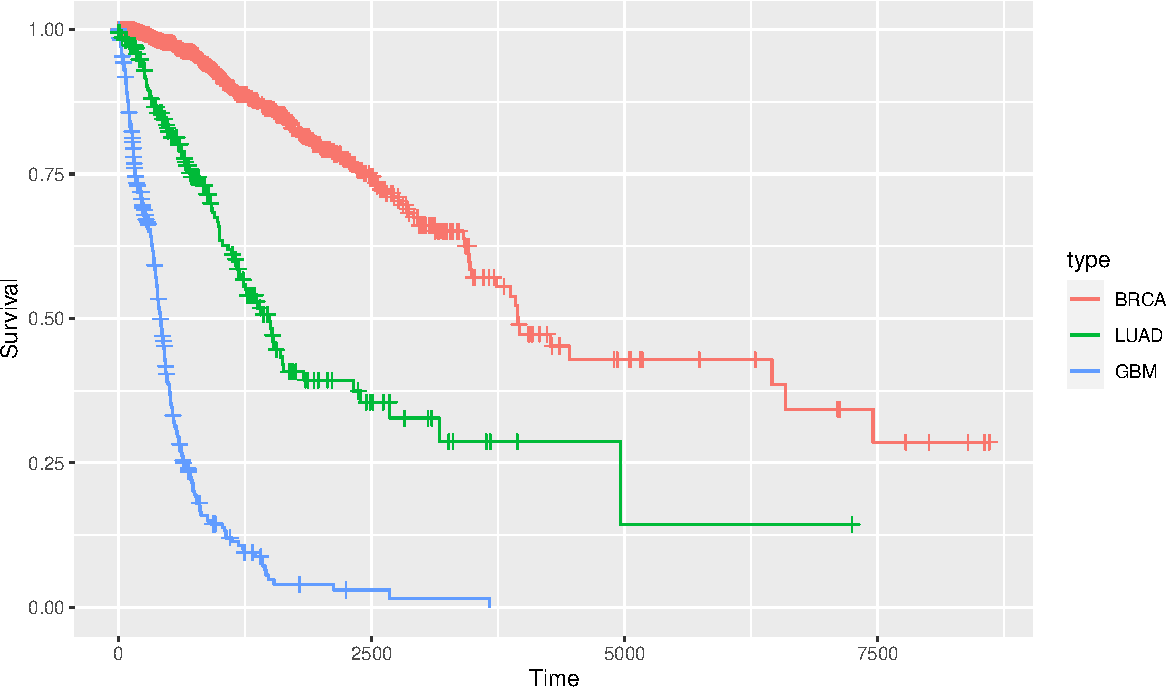
\includegraphics[width=0.8\linewidth,]{bioccb_files/figure-latex/dothesurv-1} \caption{Survival profile extraction from three MultiAssayExperiments produced with curatedTCGAData calls.}\label{fig:dothesurv}
\end{figure}

At this point, survival times within tumor type can be stratified by any
features of the mutation profiles of individual samples.
The ``RaggedExperiment'' class is employed to test each BRCA sample for
presence of any mutation in the gene TTN. See Figure \ref{fig:strat}.

\begin{shaded}
\begin{verbatim}
bprim = TCGAprimaryTumors(brmut)
## harmonizing input:
## removing 5 sampleMap rows with 'colname' not in 
##      colnames of experiments
mutsyms = assay(experiments(bprim)[[1]], "Hugo_Symbol")
cn = rownames(colData(bprim)) # short
cna = colnames(mutsyms) # long
cnas = substr(cna, 1, 12)
hasTTNmut = apply(assay(experiments(TCGAprimaryTumors(brmut))[[1]], 
     "Hugo_Symbol"), 2, function(x) length(which(x=="TTN"))>0)
## harmonizing input:
## removing 5 sampleMap rows with 'colname' not in
##      colnames of experiments
names(hasTTNmut) = cnas
bsurv = getSurv(TCGAprimaryTumors(brmut))
## harmonizing input:
## removing 5 sampleMap rows with 'colname' not in 
##      colnames of experiments
hasTTNmut = hasTTNmut[cn] # match mutation records to surv times
ggsurv(survfit(bsurv~hasTTNmut))
\end{verbatim}
\end{shaded}


\begin{figure}
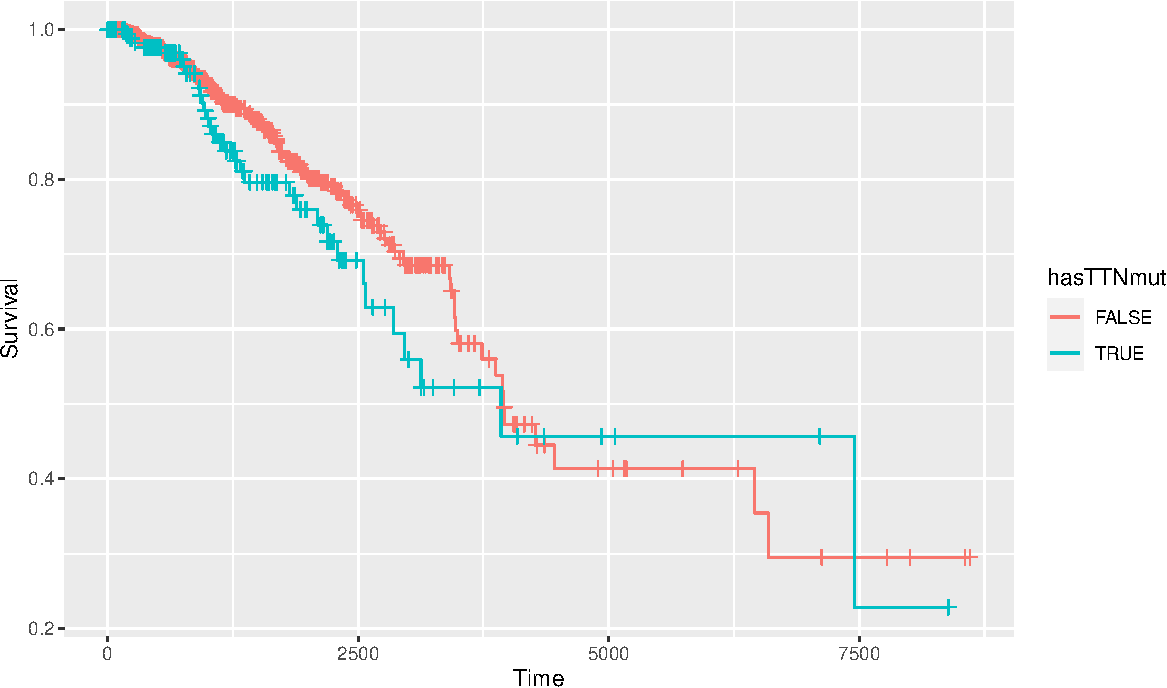
\includegraphics[width=1\linewidth,]{bioccb_files/figure-latex/strat-1} \caption{Survival distributions for donors of breast tumors in TCGA, stratified by presence or absence of mutation in gene TTN.}\label{fig:strat}
\end{figure}

Similar manipulations permit exploration of relationships between
any molecular assay outcomes and any clinical data collected in TCGA.


\subsection{cBioPortal}\label{cbioportal}}

The cBioPortal user guide
at 
\begin{verbatim}
https://www.cbioportal.org/
\end{verbatim}
defines the goal of the portal to be reducing ``the barriers between complex
genomic data and cancer researchers by providing rapid, intuitive, and high-quality
access to molecular profiles and clinical attributes from large-scale cancer genomics projects, and
therefore to empower researchers to translate these rich data sets into biologic insights and clinical applications.''

Bioconductor's cBioPortalData package simplifies access to over 300 genomic studies of
diverse cancers in cBioPortal. The main unit of data access is the publication. The
\texttt{cBioPortal} function mediates a connection between an R session and the
cBioPortal API. \texttt{getStudies} returns a tibble with metadata on
all studies.

\begin{shaded}
\begin{verbatim}
library(cBioPortalData)
cbio = cBioPortal()
allst = getStudies(cbio)
dim(allst)
## [1] 397 13
\end{verbatim}
\end{shaded}

A pruned selection of records from the cBioPortal
studies table is given in Table \ref{tab:tab-cball}.

\begin{table}
\caption{\label{tab:tab-cball}Excerpts from four fields on selected records in the cBioPortal getStudies output.}\\
\begin{tabular}{p{5cm}p{5cm}l}
name & description & studyId \\ \hline
Adenoid Cystic Carcinoma of the Breast & Whole exome sequencing of 12 breast AdCCs. & acbc\_mskcc\_2015 \\
Adenoid Cystic Carcinoma & Whole-exome or whole-genome sequencing analysis of 60 ACC tumor/normal pairs & acyc\_mskcc\_2013 \\
Adenoid Cystic Carcinoma & Targeted Sequencing of 28 metastatic Adenoid Cystic Carcinoma samples. & acyc\_fmi\_2014 \\
Adenoid Cystic Carcinoma & Whole-genome or whole-exome sequencing of 25 adenoid cystic carcinoma tumor/normal pairs. & acyc\_jhu\_2016 \\
Adenoid Cystic Carcinoma & WGS of 21 salivary ACCs and targeted molecular analyses of a validation set (81 patients). & acyc\_mda\_2015 \\
Adenoid Cystic Carcinoma & Whole-genome/exome sequencing of 10 ACC PDX models. & acyc\_mgh\_2016 \\
Adenoid Cystic Carcinoma & Whole exome sequencing of 24 ACCs. & acyc\_sanger\_2013 \\
Adenoid Cystic Carcinoma Project & Multi-Institute Cohort of 1045 Adenoid Cystic Carcinoma patients. & acc\_2019 \\
Basal Cell Carcinoma & Whole-exome sequencing of 126 basal cell carcinoma tumor/normal pairs; targeted sequencing of 163 sporadic samples (40 tumor/normal pairs) and 4 Gorlin symdrome basal cell carcinomas. & bcc\_unige\_2016 \\
\end{tabular}
\end{table}

%\begin{table}[lll]%{>{\raggedright\arraybackslash}p{12em}>{\raggedright\arraybackslash}p{15em}l}
%\caption{\label{tab:tab-cball}Excerpts from four fields on selected records in the cBioPortal getStudies output.}\\
%\toprule
%name & description & studyId\\
%\midrule
%Adenoid Cystic Carcinoma of the Breast & Whole exome sequencing of 12 breast AdCCs. & acbc\_mskcc\_2015\\
%Adenoid Cystic Carcinoma & Whole-exome or whole-genome sequencing analysis of 60 ACC tumor/normal pairs & acyc\_mskcc\_2013\\
%Adenoid Cystic Carcinoma & Targeted Sequencing of 28 metastatic Adenoid Cystic Carcinoma samples. & acyc\_fmi\_2014\\
%Adenoid Cystic Carcinoma & Whole-genome or whole-exome sequencing of 25 adenoid cystic carcinoma tumor/normal pairs. & acyc\_jhu\_2016\\
%Adenoid Cystic Carcinoma & WGS of 21 salivary ACCs and targeted molecular analyses of a validation set (81 patients). & acyc\_mda\_2015\\
%\addlinespace
%Adenoid Cystic Carcinoma & Whole-genome/exome sequencing of 10 ACC PDX models. & acyc\_mgh\_2016\\
%Adenoid Cystic Carcinoma & Whole exome sequencing of 24 ACCs. & acyc\_sanger\_2013\\
%Adenoid Cystic Carcinoma Project & Multi-Institute Cohort of 1045 Adenoid Cystic Carcinoma patients. & acc\_2019\\
%Basal Cell Carcinoma & Whole-exome sequencing of 126 basal cell carcinoma tumor/normal pairs; targeted sequencing of 163 sporadic samples (40 tumor/normal pairs) and 4 Gorlin symdrome basal cell carcinomas. & bcc\_unige\_2016\\
%\bottomrule
%\end{table}

To explore copy number alteration data from a study on angiosarcoma,
we find the associated studyId field in \texttt{allst} and use the \texttt{cBioDataPack} function
to retrieve a MultiAssayExperiment:

\begin{shaded}
\begin{verbatim}
ann = "angs_project_painter_2018"
ang = cBioDataPack(ann)
ang
## A MultiAssayExperiment object of 3 listed
##experiments with user-defined names and respective classes.
####Containing an ExperimentList class object of length 3:
##[1] cna_hg19.seg: RaggedExperiment with 27835 rows and 48 columns
##[2] cna: SummarizedExperiment with 23109 rows and 48 columns
##[3] mutations: RaggedExperiment with 24058 rows and 48 columns
## Functionality:
##experiments() - obtain the ExperimentList instance
##colData() - the primary/phenotype DataFrame
##sampleMap() - the sample coordination DataFrame
##`$`, `[`, `[[` - extract colData columns, subset, or experiment
####*Format() - convert into a long or wide DataFrame
assays() - convert ExperimentList to a SimpleList of matrices
##exportClass() - save data to flat files
\end{verbatim}
\end{shaded}

The copy number alteration outcomes are in the
\texttt{assay} component of the experiment.

\begin{shaded}
\begin{verbatim}
seg = experiments(ang)[[1]]
colnames(seg) = sapply(strsplit(colnames(seg), "-"), "[", 5)
assay(seg)[1:4,1:4]
##
##                   DAE1F DACME DADBW DAD34
## 1:12227-955755       71    NA    NA    NA
## 1:957844-1139868     62    NA    NA    NA
## 1:1140874-1471177   167    NA    NA    NA
## 1:1475170-1855370   113    NA    NA    NA
\end{verbatim}
\end{shaded}

The rownames component of this matrix can be transformed to
a GenomicRanges instance for concise manipulation.

\begin{shaded}
\begin{verbatim}
allalt = GRanges(rownames(assay(seg)))
 allalt
## GRanges object with 27835 ranges and 0 metadata columns:
##           seqnames            ranges strand
##              <Rle>         <IRanges>  <Rle>
##       [1]        1      12227-955755      *
##       [2]        1    957844-1139868      *
##       [3]        1   1140874-1471177      *
##       [4]        1   1475170-1855370      *
##       [5]        1  1857786-17257894      *
##       ...      ...               ...    ...
##   [27831]       20     68410-1559342      *
##   [27832]       20   1585705-1592359      *
##   [27833]       20  1616247-62904955      *
##   [27834]       21  9907492-48084286      *
##   [27835]       22 16157938-51237572      *
##   -------
##   seqinfo: 22 sequences from an unspecified genome; no seqlengths
\end{verbatim}
\end{shaded}


We'll focus on chromosome 17, where TP53 is found. Regions
of genomic alteration are summarized to their midpoints.
The display in Figure \ref{fig:mkden} shows a strong peak in the vicinity of 7.5 Mb on chromosome 17, near TP53.

\begin{shaded}
\begin{verbatim}
g17 = allalt[seqnames(allalt)=="17"]
df17 = as(g17, "data.frame")
df17$mid = .5*(df17$start+df17$end) # midpoint only
ggplot(df17, aes(x=mid)) + geom_density(bw=.2) + xlab("chr 17 bp")
\end{verbatim}
\end{shaded}


\begin{figure}
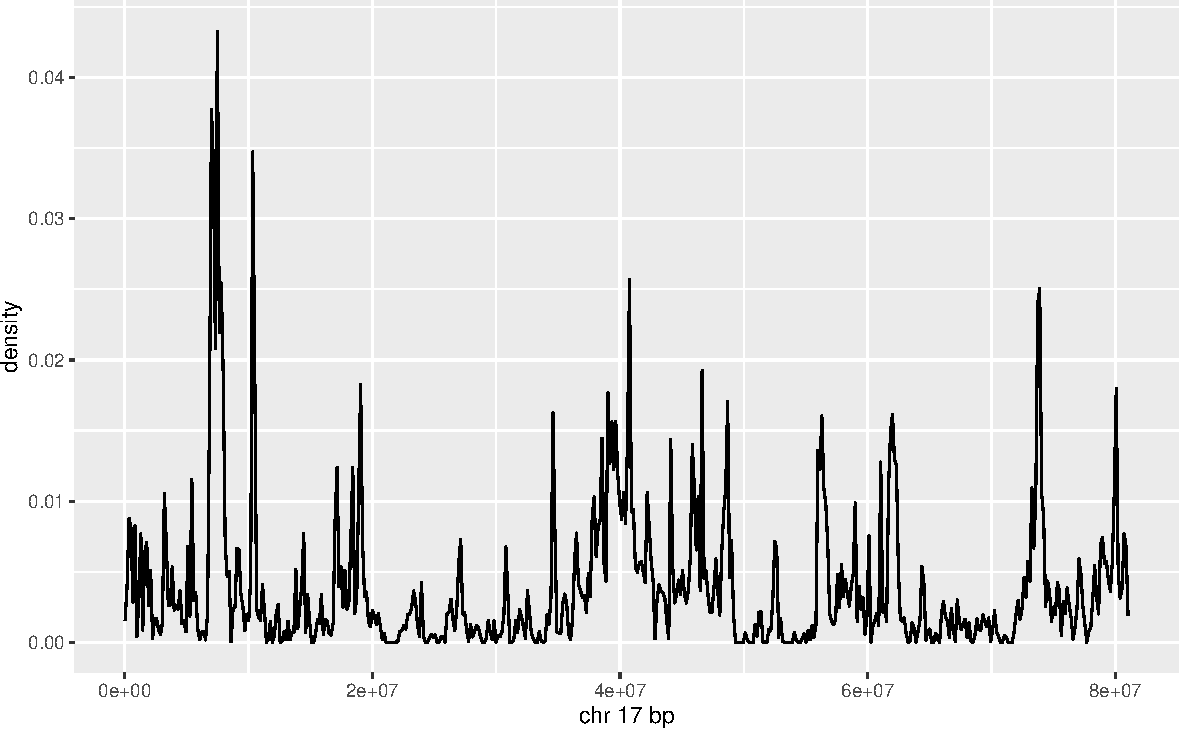
\includegraphics[width=1\linewidth,]{bioccb_files/figure-latex/mkden-1} \caption{Density of recurrent genomic alterations on chromosome 17 for 48 angiosarcoma patients.}\label{fig:mkden}
\end{figure}



\section{Genomic annotation resources relevant to cancer}\label{hubs}


\subsection{Resources from UCSC, NCBI, and EMBL}\label{resources-from-ucsc-ncbi-and-embl}

Sequences for reference genome builds for human and
other model organisms are supplied in BSgenome packages.
BSgenome.Hsapiens.UCSC.hg19 provides all chromosomes and
contigs for the 2009 build; the hg38 suffix may be used
for the 2013 build. The recent ``telomere to telomere''
build is available as BSgenome.Hsapiens.NCBI.T2T.CHMv13v2.0.

NCBI's dbSNP catalog of genetic variants is provided
in versioned packages.
For example, SNPlocs.Hsapiens.dbSNP155.GRCh38 includes
position and nucleotide content information for over
1 billion SNP identifiers ("rs numbers").

Tracks defined for the UCSC genome browser are also
packaged. The package 
\begin{verbatim}
TxDb.Hsapiens.UCSC.knownGene.hg38 
\end{verbatim} 
can be
used to get gene, transcript, and exon location information
for the hg38 build. The EnsDb packages provide similar
information for annotations curated at EMBL.

%\begin{shaded}
%\KeywordTok{library}\NormalTok{(EnsDb.Hsapiens.v86)}
%\NormalTok{EnsDb.Hsapiens.v86}
%\CommentTok{\#\# EnsDb for Ensembl:}
%\CommentTok{\#\# |Backend: SQLite}
%\CommentTok{\#\# |Db type: EnsDb}
%\CommentTok{\#\# |Type of Gene ID: Ensembl Gene ID}
%\CommentTok{\#\# |Supporting package: ensembldb}
%\CommentTok{\#\# |Db created by: ensembldb package from Bioconductor}
%\CommentTok{\#\# |script\_version: 0.3.0}
%\CommentTok{\#\# |Creation time: Thu May 18 16:32:27 2017}
%\CommentTok{\#\# |ensembl\_version: 86}
%\CommentTok{\#\# |ensembl\_host: localhost}
%\CommentTok{\#\# |Organism: homo\_sapiens}
%\CommentTok{\#\# |taxonomy\_id: 9606}
%\CommentTok{\#\# |genome\_build: GRCh38}
%\CommentTok{\#\# |DBSCHEMAVERSION: 2.0}
%\CommentTok{\#\# | No. of genes: 63970.}
%\CommentTok{\#\# | No. of transcripts: 216741.}
%\CommentTok{\#\# |Protein data available.}
%\end{Highlighting}
%\end{shaded}

\begin{shaded}
\begin{verbatim}
library(EnsDb.Hsapiens.v86)
EnsDb.Hsapiens.v86
## EnsDb for Ensembl:
## |Backend: SQLite
## |Db type: EnsDb
## |Type of Gene ID: Ensembl Gene ID
## |Supporting package: ensembldb
## |Db created by: ensembldb package from Bioconductor
## |script\_version: 0.3.0
## |Creation time: Thu May 18 16:32:27 2017
## |ensembl\_version: 86
## |ensembl\_host: localhost
## |Organism: homo\_sapiens
## |taxonomy\_id: 9606
## |genome\_build: GRCh38
## |DBSCHEMAVERSION: 2.0
## | No. of genes: 63970.
## | No. of transcripts: 216741.
## |Protein data available.
\end{verbatim}
\end{shaded}


The ``genes'' method provides addresses and additional
annotations.

\begin{shaded}
\begin{verbatim}
names(mcols(genes(EnsDb.Hsapiens.v86)))
## [1] "gene_id"          "gene_name"        "gene_biotype"     
## [4] "seq_coord_system" "symbol"           "entrezid"
head(table(genes(EnsDb.Hsapiens.v86)$gene_biotype))
##      3prime_overlapping_ncRNA                     antisense 
##                            30                          5703 
## bidirectional_promoter_lncRNA                     IG_C_gene 
##                             4                            23 
##               IG_C_pseudogene                     IG_D_gene 
##                            11                            64
\end{verbatim}
\end{shaded}

More recent versions of Ensembl gene annotation are available
from AnnotationHub, as illustrated above in section \ref{cache} with
the creation of \texttt{ens110}.

\subsection{Gene sets}\label{gene-sets}

Many methods have been developed to employ collections
of genes for inference on hypotheses about cancer
initiation or progression. The Molecular Signatures Database (MSigDB)
is curated at Broad Institute, and can be harvested
using the msigdb package.

Collect all gene sets for humans:

\begin{shaded}
\begin{verbatim}
library(msigdb)
hssigs = getMsigdb(org="hs", id="SYM", version=getMsigdbVersions())
\end{verbatim}
\end{shaded}

Find those with CANCER in their name:

\begin{shaded}
\begin{verbatim}
nms = grep("CANCER", names(hssigs), value=TRUE)
head(nms)
## [1] "SOGA_COLORECTAL_CANCER_MYC_DN"
## [2] "SOGA_COLORECTAL_CANCER_MYC_UP"
## [3] "WATANABE_RECTAL_CANCER_RADIOTHERAPY_RESPONSIVE_UP"
## [4] "LIU_PROSTATE_CANCER_UP"
## [5] "BERTUCCI_MEDULLARY_VS_DUCTAL_BREAST_CANCER_UP"
## [6] "WATANABE_COLON_CANCER_MSI_VS_MSS_UP"
wangmet = hssigs[["WANG_METASTASIS_OF_BREAST_CANCER_ESR1_UP"]]
wangmet
## setName: WANG_METASTASIS_OF_BREAST_CANCER_ESR1_UP
## geneIds: KPNA2, HDGFL3, ..., PSMC2 (total: 22)
## geneIdType: Symbol
## collectionType: Broad
##bcCategory: c2 (Curated)
##bcSubCategory: CGP
## details: use 'details(object)'
\end{verbatim}
\end{shaded}

Information on provenance is bound together with the gene list:

\begin{shaded}
\begin{verbatim}
details(wangmet)
## setName: WANG_METASTASIS_OF_BREAST_CANCER_ESR1_UP
## geneIds: KPNA2, HDGFL3, ..., PSMC2 (total: 22)
## geneIdType: Symbol
## collectionType: Broad
##bcCategory: c2 (Curated)
##bcSubCategory: CGP
## setIdentifier: LVY1HGGWMJ7:35020:Fri May 26 13:33:02 2023:1104005
## description: Genes whose expression in primary ER(+) 
##      [GeneID=2099] breast cancer tumors positively correla
## (longDescription available)
## organism: Homo sapiens
## pubMedIds: 15721472
## urls: https://data.broadinstitute.org/gsea-msigdb/msigdb/
##    release/2023.1.Hs/msigdb_v2023.1.Hs.xml.zip
## contributor: Arthur Liberzon
\end{verbatim}
\end{shaded}

\subsection{Ontologies}\label{ontologies}

Informal reasoning about cancer genomics employs conventional
but frequently ambiguous terminology. In modern
information science, ontologies are structured vocabularies
(sets of ``terms'', which may be single words or natural language
phrases) accompanied by
explicit statements of semantic relationships among terms.

Bioconductor provides several approaches for using ontologies
in cancer data science. The most familiar ontology
in this domain is Gene Ontology (GO), which organizes vocabulary
about genes and gene products in
the areas of molecular function, cellular components, and
biological processes.

\subsubsection{Ontology usage with AnnotationDbi}\label{ontology-usage-with-annotationdbi}

A common use case is to find genes or proteins associated
with some biological process, component, or function.
A phrase like `Golgi membrane' can be found in Gene Ontology
using the select method with GO.db:

\begin{shaded}
\begin{verbatim}
library(GO.db)
select(GO.db, keytype="TERM",
keys="Golgi membrane", columns=c("GOID", "DEFINITION", "ONTOLOGY"))
##             TERM       GOID
## 1 Golgi membrane GO:0000139
##                                 DEFINITION
## 1 The lipid bilayer surrounding any of the 
## compartments of the Golgi apparatus.
## ONTOLOGY
## 1     CC
\end{verbatim}
\end{shaded}

Once the formal identifier is obtained, the org.Hs.eg.db package can be used to find mappings
from the GO term to gene and protein identifiers. This generates a fairly large table:

\begin{shaded}
\begin{verbatim}
library(org.Hs.eg.db)
go139 = select(org.Hs.eg.db, keys="GO:0000139", keytype="GO",
columns=c("ENTREZID", "SYMBOL", "PFAM"))
dim(go139)
## [1] 1212 6
head(go139)
##           GO EVIDENCE ONTOLOGY ENTREZID SYMBOL    PFAM
## 1 GO:0000139      TAS       CC       28    ABO PF03414
## 2 GO:0000139      IEA       CC      102 ADAM10 PF00200
## 3 GO:0000139      IEA       CC      102 ADAM10 PF13574
## 4 GO:0000139      IEA       CC      102 ADAM10 PF01562
## 5 GO:0000139      TAS       CC      162  AP1B1 PF09066
## 6 GO:0000139      TAS       CC      162  AP1B1 PF01602
\end{verbatim}
\end{shaded}

The evidence code TAS means that there is a ``traceable author statement'' associating the term
of interest with the gene identified. The number of genes in traceable Golgi membrane:gene
associations is found with

\begin{shaded}
\begin{verbatim}
go139 |> dplyr::filter(EVIDENCE=="TAS") |> distinct(ENTREZID) |> count()
##       n
## [1] 327
\end{verbatim}
\end{shaded}


\subsubsection{Ontology usage with rols}\label{ontology-usage-with-rols}

Access to a vast collection of ontologies is afforded by the EBI's
Ontology Lookup Service (OLS). The rols package uses the OLS API
to discover ontologic mapping of terms of interest. Here we'll
consider the term ``golgi membrane dynamics'', which is not found in GO.
Again a multistep process is used.

\begin{shaded}
\begin{verbatim}
library(rols)
lk1 = OlsSearch(q="golgi membrane dynamics", exact=TRUE)
lk1
## Object of class 'OlsSearch':
##query: golgi membrane dynamics
##requested: 20 (out of 3)
##response(s): 0
\end{verbatim}
\end{shaded}


In this first step, we find how extensive is the response
to the query. Certain searches yield tens of thousands of hits.
With the exact parameter setting, the yield is modest.
Now we extract a data.frame after requesting all
records with \texttt{olsSearch}.  Results are
excerpted in Table \ref{tab:tab-golg}.

\begin{shaded}
\begin{verbatim}
lk2 = olsSearch(lk1)
lk3 = as(lk2, "data.frame")
lk3$description = unlist(lk3$description)
\end{verbatim}
\end{shaded}



\begin{table}
\caption{Using rols to obtain ontologic information related to
golgi membrane dynamics. \label{tab:tab-golg}}
\begin{tabular}{lp{5cm}p{8cm}}
\toprule
short\_form & description & label\\
\midrule
NCIT\_C119637 & This gene is involved in both protein ubiquitination and Golgi membrane dynamics. & HACE1 Gene\\
NCIT\_C119639 & E3 ubiquitin-protein ligase HACE1 (909 aa, \textasciitilde{}102 kDa) is encoded by the human HACE1 gene. This protein is involved in the regulation of both the ubiquitination and subsequent degradation of small GTPases, which modulates Golgi membrane dynamics. & E3 Ubiquitin-Protein Ligase HACE1\\
NCIT\_C119638 & Human HACE1 wild-type allele is located in the vicinity of 6q16.3 and is approximately 132 kb in length. This allele, which encodes E3 ubiquitin-protein ligase HACE1 protein, plays a role in the modulation of both Golgi membrane dynamics and ubiquitination. Mutations of the gene, including translocations that either reduce expression of the gene (t(6;15)(q21;q21)) or truncate the gene (t(5;6)(q21;q21)), are associated with Wilms tumor. & HACE1 wt Allele\\
\bottomrule
\end{tabular}
\end{table}

The detailed descriptions of the NCI Thesaurus entries show
the exact nature of the search outcome.

\subsubsection{Cross-ontology relationships}\label{cross-ontology-relationships}

Philosophically, ontology is the study of what there is. For
applications in information
science,
boundaries need to be established so that ontological
resources can be managed with well-defined scopes. In Gene
Ontology, three sub-ontologies are explicitly identified for
cellular components, biological processes, and molecular functions.

As knowledge of cell biology increases, the typology of
cells becomes more and more intricate. Differentiation
and definition
of ``cell types'' involves concepts from immunology,
protein science, anatomy, and other conceptual domains
for which ontologies have been developed. Figure \ref{fig:ontopair}
presents, on the left, the hierarchy of cell type concepts starting at ``lymphocyte'',
leading to ``Type II Natural Killer T cell secreting interferon gamma''.
On the right, some of the GO and Protein Ontology (PR) cross-references
in the Cell Ontology (CL) entry for the Type II NK cell are shown.
The ``cond'' column of the table contains abbreviated tokens
representing formal relationships linking the cell type
to the protein or cellular component elements of PR and GO.
The token ``hasPMP'' refers to the element of the Relation Ontology
(RO) ``has plasma membrane part'' (RO:0002104).

\begin{figure}
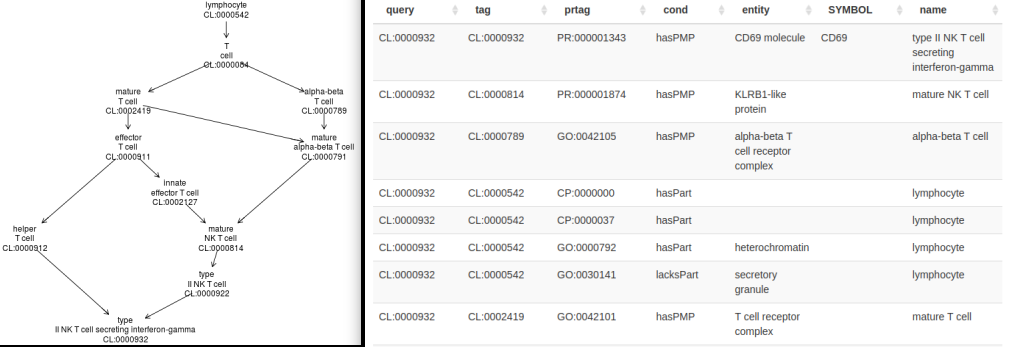
\includegraphics[width=1\linewidth,]{ontoPair} \caption{Ontology visualization and tabulation with ontoProc::ctmarks.}\label{fig:ontopair}
\end{figure}

Prospects for use of ontological discipline in the
definition of new cell types are reviewed in a 2018
paper from the Venter Institute \cite{Aevermann2018}.

The field of biological ontology is rapidly advancing,
and the integration of ontology search and inference
with data analytic frameworks requires more effort at this time.

